\documentclass{article}


\usepackage{arxiv}

\usepackage[utf8]{inputenc} % allow utf-8 input
\usepackage[T1]{fontenc}    % use 8-bit T1 fonts
\usepackage{hyperref}       % hyperlinks
\usepackage{url}            % simple URL typesetting
\usepackage{booktabs}       % professional-quality tables
\usepackage{amsfonts}       % blackboard math symbols
\usepackage{nicefrac}       % compact symbols for 1/2, etc.
\usepackage{microtype}      % microtypography
\usepackage{lipsum}		% Can be removed after putting your text content
\usepackage{textgreek}
\usepackage{amsmath}
\usepackage{algorithm}
\usepackage{algpseudocode}
\usepackage{algpascal}
\usepackage{graphicx}
\usepackage[
backend=biber,
style=numeric,
sorting=ynt,
citestyle=authoryear
]{biblatex}
\addbibresource{paper.bib}

%\graphicspath{ {./images/} }

\title{Replicating Greenwald and Hall's Correlated-Q Learning in Soccer}

\date{July 21st, 2019}

\author{
Carlos Souza\thanks{Latest Git hash: INCLUDE LATEST GITHASH}\\
%Department of Computer Science\\
Georgia Institute of Technology\\
São Paulo, SP, Brazil \\
\texttt{souza@gatech.edu} \\
}

\DeclareMathOperator*{\argmax}{arg\,max}
\DeclareMathOperator*{\argmin}{arg\,min}


\begin{document}
    \maketitle

    \begin{abstract}
        \lipsum[1]
    \end{abstract}

    % keywords can be removed
    \keywords{Reinforcement learning \and Correlated-Q learning \and Markov games \and Nash equilibrium \and Correlated equilibrium}

    \section{Introduction}
    \label{sec:introduction}
    In 2003, Greenwald  and Hall introduced Correlated-Q (CE-Q) learning (\cite{greenwald2003}), a multiagent Q-learning algorithm based on the correlated equilibrium solution concept designed to learn equilibrium policies in general-sum Markov games.
    This algorithm generalized both Hu and Wellman's Nash-Q algorithm (\cite{hu1998}), which converges to Nash equilibrium policies under restrictive conditions, and Littman's friend-or-foe-Q (FF-Q) algorithm (\cite{littman2001}), which always converges but only works in restricted classes of games (e.g. two-player, constant-sum Markov games, which exhibit minimax equilibria).
    The purpose of this paper is to discuss the results obtained by replicating four algorithms implemented and tested in soccer environment as described by Greenwald and Hall, providing a complete description of the experiments, implementation details and outcomes.

    \subsection{Background}
    \label{subsec:background}
    A Markov Decision Process (MDP) is a tuple $\langle \mathcal{S}, \mathcal{A}, P, R, \gamma \rangle$, where $\mathcal{S}$ is a finite set of states, $\mathcal{A}$ is a finite set of actions, $P$ is a state transition probability matrix, $R$ is a reward function and $\gamma$ is the discount factor.

    In a MDP, the agent's objective is to find a policy $\pi$ that maximizes the expected sum of discounted rewards:

    \begin{equation}
        v(s, \pi) = \sum_{t=0}^{\infty} \gamma^{t} \; \mathbb{E}(r_{t} \; | \; s_{0} = s)
    \end{equation}

    where $s_{0}$ is the initial state and $r_{t}$ is the reward at time $t$.

    It has been proved that there is an optimal policy $\pi^{*}$ such that, for any $s \in \mathcal{S}$, Bellman equation holds:

    \begin{equation}
        v(s, \pi^{*}) = \max_{a} \left ( r(s, a) + \gamma \sum_{s'} p(s' \; | \; s, a) \; v(s', \pi^{*}) \right)
    \end{equation}

    Finding the optimal policy $\pi^{*}$ can be done using iterative searching methods when reward and state transition functions are known.
    When these functions are not know, the agent can either learn them by interacting with the environment and use the equations above to solve for $\pi^{*}$ (model-based reinforcement learning), or directly learn the optimal policy (model-free reinforcement learning).
    One of the most popular model-free reinforcement learning methods is \emph{Q-learning}.
    Key equations of this method are:
    \begin{align}
        Q^{*}(s, a) &= r(s, a) + \gamma \sum_{s'} p(s' \; | \; s, a) \; v(s', \pi^{*}) \\
        v(s, \pi^{*}) &= \max_a Q^{*}(s, a) \\
        \pi^{*}(s) &\in \argmax_a Q^{*}(s, a) \label{eq1}
    \end{align}

    Given $Q^{*}(s, a)$, the optimal policy $\pi^{*}$ can be found by always taking the action $a \in \mathcal{A}$ that maximizes $Q^{*}(s, a)$ for all $s \in \mathcal{S}$.
    In Q-learning, at each time step $t$ the agent interacts with the environment and updates its estimate of $Q$ based on the following equation:
    \begin{equation}
        Q_{t+1}(s, a) = (1 - \alpha_{t}) Q_{t} + \alpha_{t} \left( r_{t} + \gamma \max_{a'} Q_{t}(s', a') \right)
    \end{equation}

    It has been proved that the above equation converges to the optimal $Q^{*}(s, a)$ when learning rate $\alpha_{t}$ decays over time.

    \subsection{Markov Games}
    \label{subsec:games}

    MDPs are single-agent decision problems.
    Markov Games are essentially n-agent Markov Decision Processes.
    They generalize MDPs and repeated games.
    Mathematically they are defined by the tuple $\langle I, \mathcal{S}, (\mathcal{A}_{i})_{1 \leq i \leq n}, P, (R_{i})_{1 \leq i \leq n}, \gamma \rangle$, where $I$ is a set of $n$ players, $\mathcal{S}$ is the state-space, $\mathcal{A}_{i}$ is the $i$th player's set of actions, $P$ is the probability transition function that describes state transitions, conditioned on past state and joint actions, and $R_{i}(s, \vec{a})$ is the $i$th player's reward for state $s \in \mathcal{S}$ and joint actions $\vec{a} \in \mathcal{A} = \mathcal{A}_{1} \times \mathcal{A}_{2} \times \ldots \times \mathcal{A}_{n}$.

    In Markov Games, player $i$'s Q-values are defined over states and action-vectors $\vec{a} = (a_{1}, a_{2}, \ldots, a_{n})$:
    \begin{equation}
        Q^{*}(s, \vec{a}) = r(s, \vec{a}) + \gamma \sum_{s'} p(s' \; | \; s, \vec{a}) \; v(s', \pi^{*})
    \end{equation}

    Although we can carry over the notion of state-value function from MDPs to Markov Games, we cannot hold Eq.\ref{eq1} true: deterministic actions that maximizes all players' rewards with respect to one another's actions may not exist.
    Several alternative definitions for the value function have been proposed.
    Here are some of them, studied in this paper.

    \paragraph{Friend-Q.}
    Littman's friend-Q value function is suited to coordination games, for which all the players' reward functions are equivalent, with uniquely-valued equilibria:
    \begin{equation}
        v_{i}(s) = \max_{\vec{a} \in \mathcal{A}} Q_{i}(s, \vec{a}) \label{eq2}
    \end{equation}

    \paragraph{Foe-Q.}
    At the opposite, Littman studied two-player, zero-sum Markov Games and von Neumann's minimax value function:
    \begin{equation}
        v_{1}(s) = \max_{\sigma_{1} \in \Sigma_{1}(s)} \min_{a_{2} \in \mathcal{A}_{2}(s)} Q_{1}(s, \sigma_{1}, a_{2}) = -v_{2}(s)
    \end{equation}
    where $\Sigma_{i}(s)$ is the probabilistic action space of player $i$ at state $s$ and $Q(s, \sigma_{1}, a_{2}) = \sum_{a_{1} \in \mathcal{A}_{1}} \sigma_{1}(a_{1}) Q(s, a_{1}, a_{2})$.

    \paragraph{Nash-Q.}
    Hu and Wellman proposed the following definition of value function for the genera case of n-player, general-sum games:
    \begin{equation}
        v_{i}(s) \in \mathsf{NASH}_{i}(Q_{1}(s), Q_{2}(s), \ldots, Q_{n}(s))
    \end{equation}
    where $\mathsf{NASH}_{i}(X_{1}, X_{2}, \ldots, X_{n})$ represents the $i$th player's reward according to some Nash equilibrium in the general-sum game determined by the reward matrices $X_{1}, X_{2}, \ldots, X_{n}$.

    \paragraph{Correlated-Q.}
    Greenwald and Hall proposed a generalization of Hu and Wellman's \emph{Nash-Q} definition:
    \begin{equation}
        v_{i}(s) \in \mathsf{CE}_{i}(Q_{1}(s), Q_{2}(s), \ldots, Q_{n}(s)) \label{eq3}
    \end{equation}
    where $\mathsf{CE}_{i}(X_{1}, X_{2}, \ldots, X_{n})$ represents the $i$th player's reward according to some \emph{correlated equilibrium} in the general-sum game determined by the reward matrices $X_{1}, X_{2}, \ldots, X_{n}$.

    A Nash equilibrium (NE) is a vector of \emph{independent} probability distributions over actions, in which all agents optimize with respect to one another's probabilities.
    A correlated equilibrium (CE), in contrast, allows for the possibility of dependencies in the agents' randomizations: a CE is a probability distribution over the \emph{joint} space of actions, in which all agents optimize with respect to one another's probabilities, conditioned on their own.

    While there is no efficient method of computing Nash equilibria, correlated equilibria can be easily computed using linear programming.

    \subsection{Multiagent Q-Learning}
    \label{subsec:mql}

    A mutiagent Q-learning algorithm generalization template from MDPs to Markov Games is presented below:

    \alglanguage{pseudocode}
    \begin{algorithm}
        \caption{Multiagent Q-Learning}
        \label{alg1}
        \begin{algorithmic}
            \Require{selection function $f$, discount factor $\gamma$, learning rate $\alpha$, total training time $T$}
            \State Initialize $s$
            \State Initialize $Q_{1}, Q_{2}, \ldots, Q_{n}$
            \State Initialize $V_{1}, V_{2}, \ldots, V_{n}$
            \For{$t \gets 1, \, T$}
                \State Agents choose actions $a_{1}, a_{2}, \ldots, a_{n}$ following $\epsilon$-greedy policy
                \State Simulate actions in state $s$
                \State Observe rewards $r_{1}, r_{2}, \ldots, r_{n}$ and next state $s'$
                \For {$i \gets 1, \, n$}
                    \State $v_{i}(s') = f_{i} \left( Q_{1}(s'), Q_{2}(s'), \ldots, Q_{n}(s') \right)$
                    \State $Q_{i}(s, \vec{a}) = (1 - \alpha) Q_{i}(s, \vec{a}) + \alpha \left[(1 - \gamma) R_{i} + \gamma \; v_{i}(s') \right]$
                \EndFor
                \State $s = s'$
                \State Decay $\alpha$ and $\epsilon$
            \EndFor
        \end{algorithmic}
    \end{algorithm}

    This algorithm takes as input an equilibrium selection function $f$, as shown previously from Eq.\ref{eq2} to Eq.\ref{eq3}.
    Specifically for correlated equilibrium, Greenwald and Hall presented four different correlated-Q learning variants, based on four different selection mechanisms.
    In the experiment section, we simulated the \emph{utilitarian} ($u$CE-Q) variant, which aims to maximize the \emph{sum} of the players' rewards:
    \begin{equation}
        \sigma \in \max_{\sigma \in \mathsf{CE}} \sum_{i \in I} \sum_{\vec{a} \in \mathcal{A}} \sigma(\vec{a}) \; Q_{i}(s, \vec{a})
    \end{equation}

    \subsection{Soccer Environment}
    \label{subsec:soccer}
    Greenwald and Hall simulated different multiagent-Q learning algorithms in a soccer grid game, a zero-sum game for which determninistic equilibrium policies do not exist.
    The soccer field is a 2-rows by 4-columns grid, as shown in Figure\ref{fig1}.
    There are two opposite players, who can choose five different actions: move North, East, South, West or stick.
    The ball, represented by the circle, is always with one of the two players.
    At each time step, both players act in random order.
    The players cannot occupy the same grid space at the same time: if the sequence of actions cause them to collide, only the first moves.
    But if the player with the ball moves \emph{second}, trying to occupy a space which is already occupied, the ball changes possession.
    If a player moves with the ball into his goal, he scores +100 and his opponent -100;
    if he moves with the ball into his opponent's goal, he scores -100, and his opponent +100.

    \begin{figure}[t]
        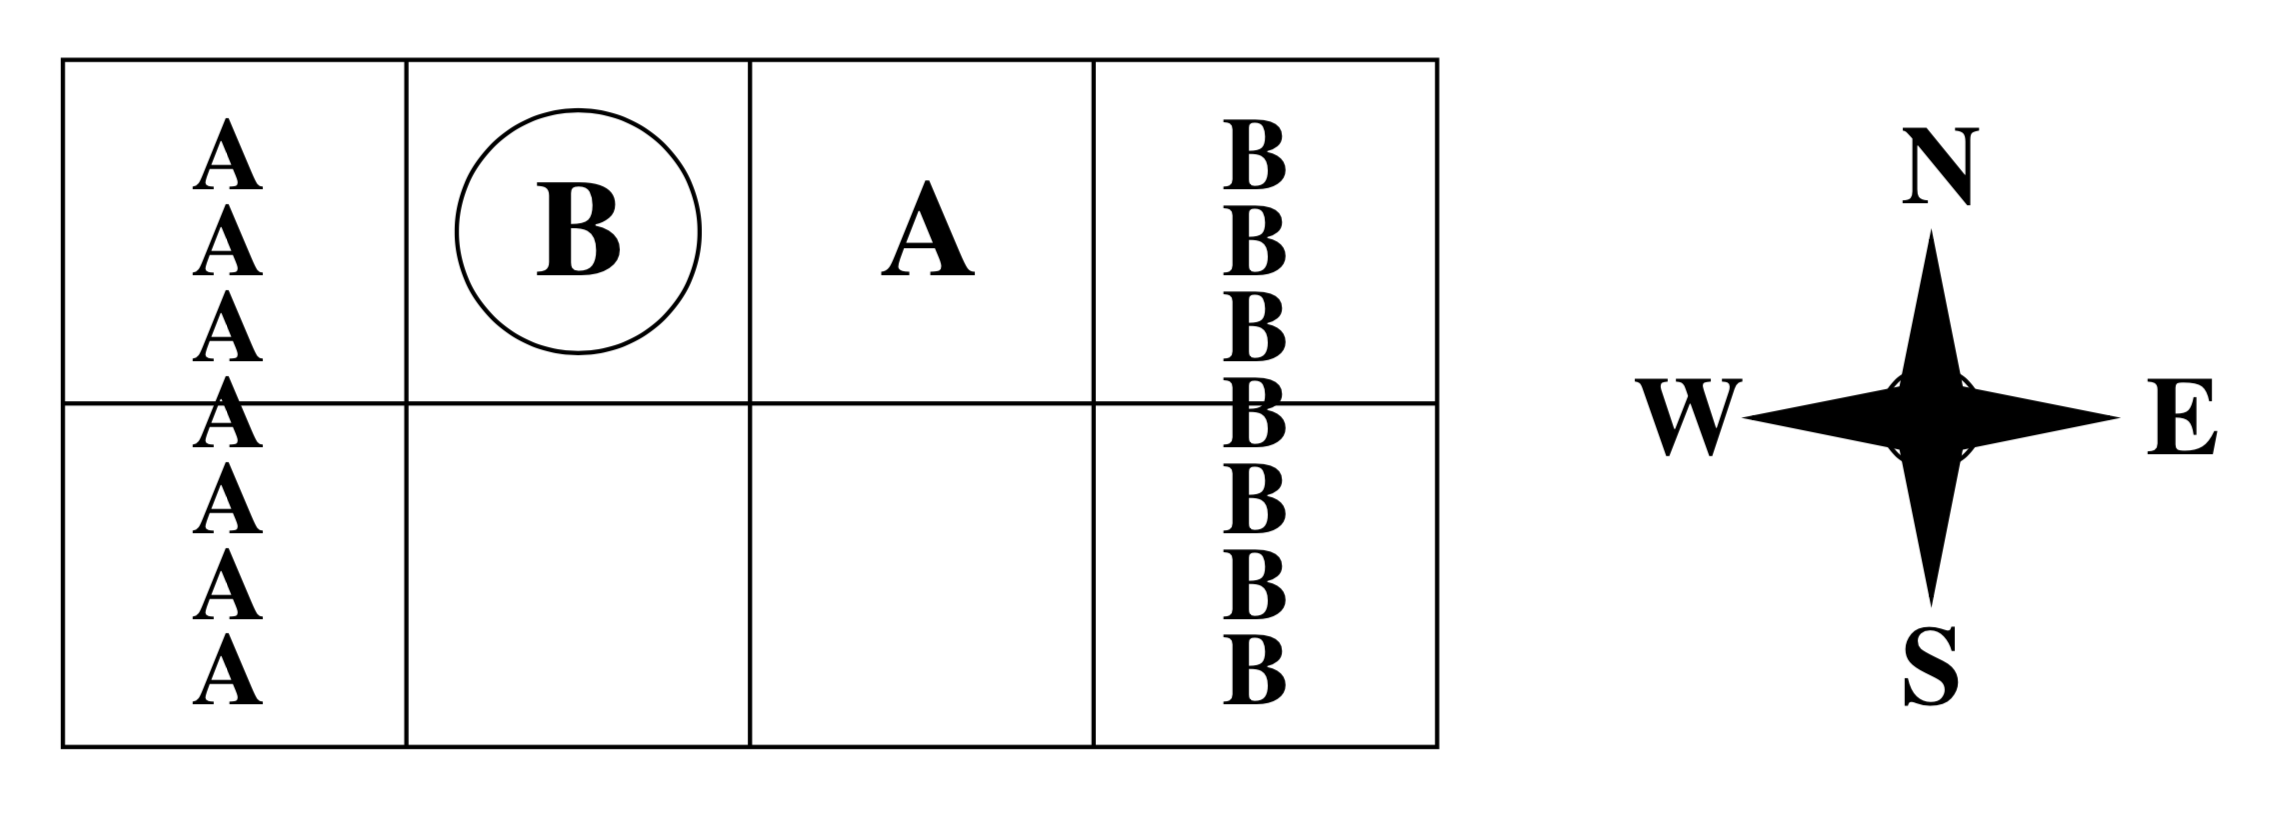
\includegraphics[scale=0.15]{./images/figure1.png}
        \centering
        \caption{Soccer Game.
        State control $s$.}
        \label{fig1}
    \end{figure}

    \section{Methods}
    \label{sec:methods}
    To replicate Greenwald and Hall's results, we followed the exact protocols described in the article.
    First, we implemented the four different algorithms shown in original article's Figure 3: Q-learning, Friend-Q, Foe-Q and Correlated-Q (utilitarian).
    We simulated $10^{6}$ time steps for each algorithm, using discount rate $\gamma = 0.9$.

    In each simulation, we decayed the learning rate $\alpha$ from $0.1$ to $0.001$, multiplying it by $0.999995$ at each time step.
    At each time step, every agent chose his action following a $\epsilon$-greedy policy: we started the simulations with $\epsilon = 1$ and decayed it until $0.001$, by also multiplying it by $0.999995$.

    To solve the linear programming set of inequalities, required in Foe-Q and uCE-Q algorithms, we used \href{https://pythonhosted.org/PuLP/}{Python's PuLP optimization package}.
    Despite its user-friendliness and fast learning curve, this library proven to be very slow in simulating the algorithms.
    For future work that requires linear programming package and a massing number of calculations, a different solution must be used, such as \href{https://cvxopt.org/}{Python's CVXOPT}.

    \section{Results}
    \label{sec:results}

    \begin{figure}[t]
        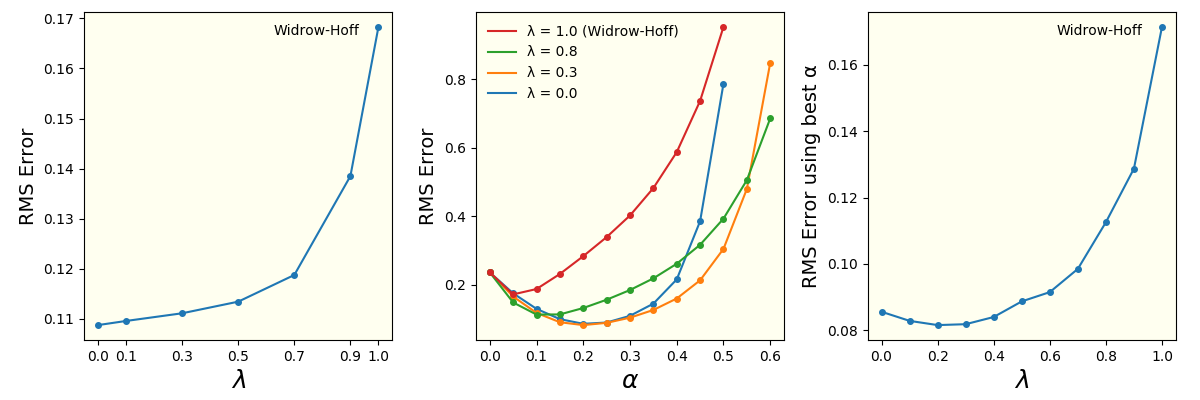
\includegraphics[width=\textwidth]{./images/figure.png}
        \centering
        \label{fig2}
        \caption{Replication of Figures 3, 4 and 5 from Sutton's original paper.
        In the left, average error on random walk problem under repeated presentations.
        In the center, average error on random walk problem after 10 episodes for different values of $\alpha$ and $\gamma$.
        In the right, average error at best $\alpha$ on random walk problem for different values of $\gamma$.}
    \end{figure}

    \lipsum[0]
    \lipsum[1]
    \lipsum[2]
    \lipsum[3]

    \section{Conclusion}
    \label{sec:conclusion}

    \lipsum[0]

\printbibliography

\end{document}
